\documentclass[11]{article}
\usepackage{graphicx}
\graphicspath{ {images/} }


\title{CS2002 Practical 2 - \\x86 Assembler}
\date{27/02/2018}
\author{Matriculation Number: 160001362}

\begin{document}
	\maketitle
	\newpage
	\tableofcontents
	
	\newpage
	\section{Overview}
	This practical specified the commenting of AT\&T x86 64-bit assembly code, the implementation of a print function to print three stack frames during the execution of a sort algorithm (and to write an analysis of the output), and an analysis of the functions of sort0.s (and how sort1.s, sort2.s, and sort3.s differ from this file). The practical also specified that as an extension the sort.c source file should be compiled for other architectures such as MIPS and ARM, and that the results should be analysed and compared with x86-64 assembly. \\\\The first stage of the practical has been achieved with the assembly in the sort-commented.s file having been commented for the sortsub function. \\\\The functionality requested by the second stage of the practical has been implemented in the stack.c file in the print\_stack and print\_frame functions which can be run in terminal by using the command ./main-plus which will print the address, offset and value of each value in each stack frame. Analysis of the results of this function can be found in the analysis section further into this report. \\\\ The third section of this practical, analysis of the functions of sort0.s and a comparison between this file and the other sort files, can also be found in the analysis section of this report. \\\\ The extension comparing MIPS and ARM assembly with x86-64 assembly is discussed under the 'extensions' heading of this report.
	\section{Design and Implementation}
	In the second section of the practical, the stack\_frame function runs an in-line assembly command to move the value stored in the base pointer register (rbp) into a local variable. This variable is then dereferenced to retrieve the value of the base pointer from the previous stack frame. My own function print\_frame is then called with the two base pointers and the number of stack frames to print as arguments. \\\\ The print\_frame function then iterates over the addresses between the previous base pointer and the current base pointer in increments of 8 bytes and prints out the address of each value, as well as its offset from the base pointer in bytes, and the value stored at the current address. The print\_frame function is then recursively called until there are no more frames to print.
	\section{Analysis}
		\subsection{Section 2 - Findings}
			\begin{figure}
				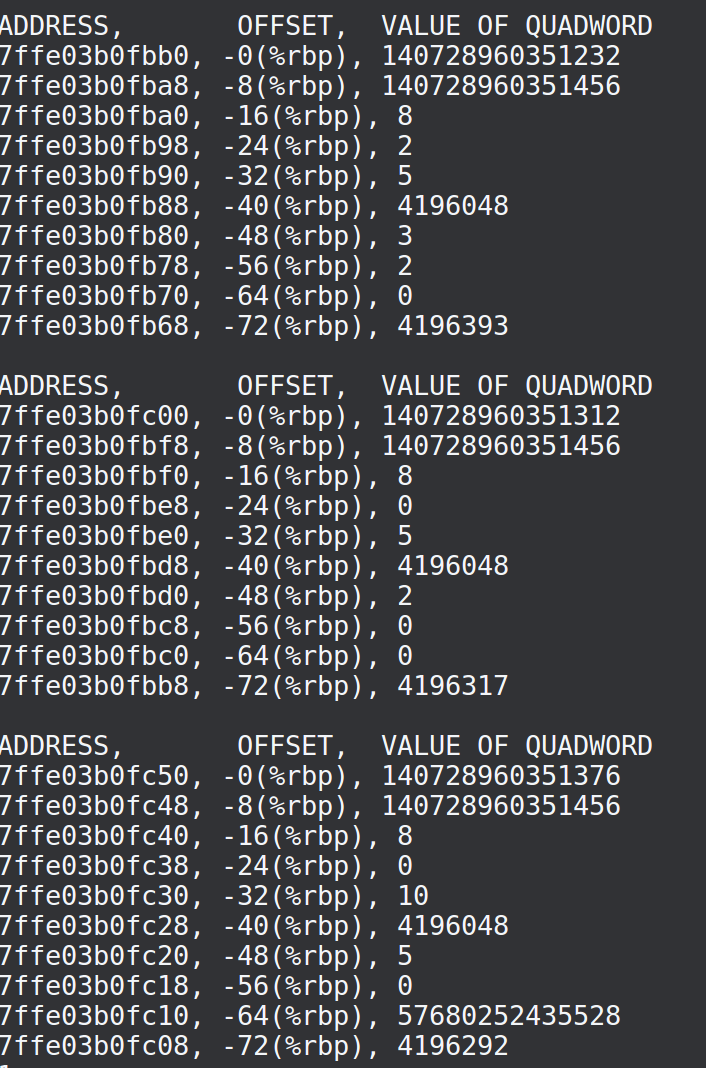
\includegraphics[scale=0.5]{Print_Stack_Output.png}
				\caption{Output of print\_stack Function}
			\end{figure}
			
			The above figure shows the terminal output of running the main-plus executable with the specified implementation of the print\_stack function. The output has been displayed in the suggested format of address, offset and value. For the most part the values output seem to correspond with values in the assembly and C code.\\\\ The first value in each stack frame is a decimal address which makes sense as it has an offset of 0 from the base pointer and therefore is the value at that current base pointer. The value in the first stack frame printed is decimal 140728960351232 which is the address of the middle stack frame in hex 7ffe03b0fc00. The second value (offset -8) is also a decimal address which corresponds to the void* array as the names of arrays in C are pointers to the first element of the array. The third, fourth and fifth values (offsets -16, -24 and -32) correspond to the size, left and right variables of type long. For the sixth value (offset -40) it appears to be the address pointing to the function comp\_long used to initialise the comp variable. However this is not certain. The seventh value output (offset -48) seems to be the value of mid which is being passed into subsort, subsort and merge respectively and is used to split the list into two smallers halves recursively. The eighth value (offset -56) is the same value as offset -24 which contains the value of left, this is because this location is where the value of left is stored before it is copied into register rcx for use in the calculation during the assignment of mid where mid = left + (right - left) / 2. 
			\subsubsection{Comparison of sort0.s and sort-plus.s}
		\subsection{Section 3}
			\subsubsection{Word Size Analysis}
			\subsubsection{Assembler Code for Comp Function Call}
			\subsubsection{Implementation of a While-Loop in Assembler}
			\subsubsection{Comparison of Sort Files}
	\section{Evaluation}
	\section{Conclusion}
	\section{Section 4 - Extension}
\end{document}